\documentclass[12pt]{article}
\usepackage{amsmath}
\usepackage{array}
% \usepackage{gensymb}
\usepackage{geometry}
\usepackage{graphicx}
\usepackage{pgfplots}
\usepackage{siunitx}
\usepackage{wrapfig}

\title{Homework \#2, 4B}
\author{Donald Aingworth IV}
\date{January 29, 2025}

\pgfplotsset{width=8cm,compat=1.9}
\usepgfplotslibrary{external}
% \tikzexternalize

\begin{document}

\DeclareSIUnit{\mile}{mi}
\DeclareSIUnit{\gal}{gal}
\DeclareSIUnit{\foot}{ft}
\DeclareSIUnit{\hour}{h}
\DeclareSIUnit{\rad}{rad}
\DeclareSIUnit{\unit}{u}
\DeclareSIUnit{\dyne}{dyn}

\maketitle

\pagebreak
\section*{Chapter 21, Problem 52}
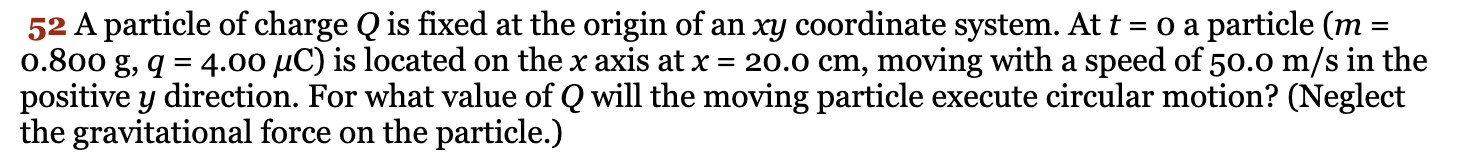
\includegraphics[width=\textwidth]{picture_1.png}

\subsection*{Solution}
Since it's rotating about a point, the electrostatic force ($F_E = \frac{kq_1 q_2}{r^2}$)must be (equal to) the centripital force, the equation for which is $F_c = \frac{mv^2}{r}$. 
\begin{gather*}
    F_E = F_c\\
    \frac{kqQ}{r^2} = \frac{mv^2}{r}
\end{gather*}
\begin{align*}
    Q   &=  \frac{mv^2r}{kq}
        =   \frac{(8.00 \times 10^{-4} \unit{\kilo\gram})(50.0\unit{\meter/\second})^2(0.2\unit{\meter})}{(8.99 \times 10^{9})(4.00 \times 10^{-6} \unit{\coulomb})}
        =   \boxed{1.112 \times 10^{-5} \unit{\coulomb}}
\end{align*}

\pagebreak
\section*{Chapter 21, Problem 66}
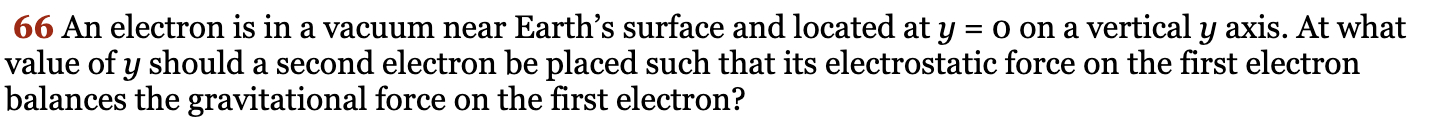
\includegraphics[width=\textwidth]{picture_2.png}

\subsection*{Solution}
In this instance, the downward gravitational force must be equal to the upwards electrostatic force, both of which we know the formulae for.
\begin{gather*}
    F_g = F_E\\
    mg = \frac{kq_1 q_2}{r^2}
\end{gather*}

We can next solve for $r$, which would be the value of the height.
\begin{gather*}
    mg = \frac{kq_1 q_2}{r^2}\\
    r^2 = \frac{k q^2}{mg}\\
    r = \sqrt{\frac{k q^2}{mg}}
\end{gather*}

We can then plug values into this answer.
\begin{align*}
    r   &=  \sqrt{\frac{k q^2}{mg}}
        =   \sqrt{\frac{(8.99 \times 10^{9} \unit{\newton\meter^2/\coulomb^2}) (1.60218 \times 10^{-19} \unit{\coulomb})^2}{(9.1093837 \times 10^{-31} \unit{\kilo\gram})(9.81 \unit{\meter/\second^2})}}\\
        &=  \sqrt{25.823938 \unit{\meter^2}}
        =   \pm 5.0817259 \unit{\meter}
\end{align*}

The earth pulls the electron downwards. So=ince the electron has the same charge as the other electron, it pushes it away rather than pulling it towards itself. As such, in order to conteract the downwards force, the second electron needs to be put below the first electron. As such, it must be that $y$ is negative, so \boxed{y = -5.0817259 \unit{\meter}}

\pagebreak
\section*{Chapter 22, Question 4}
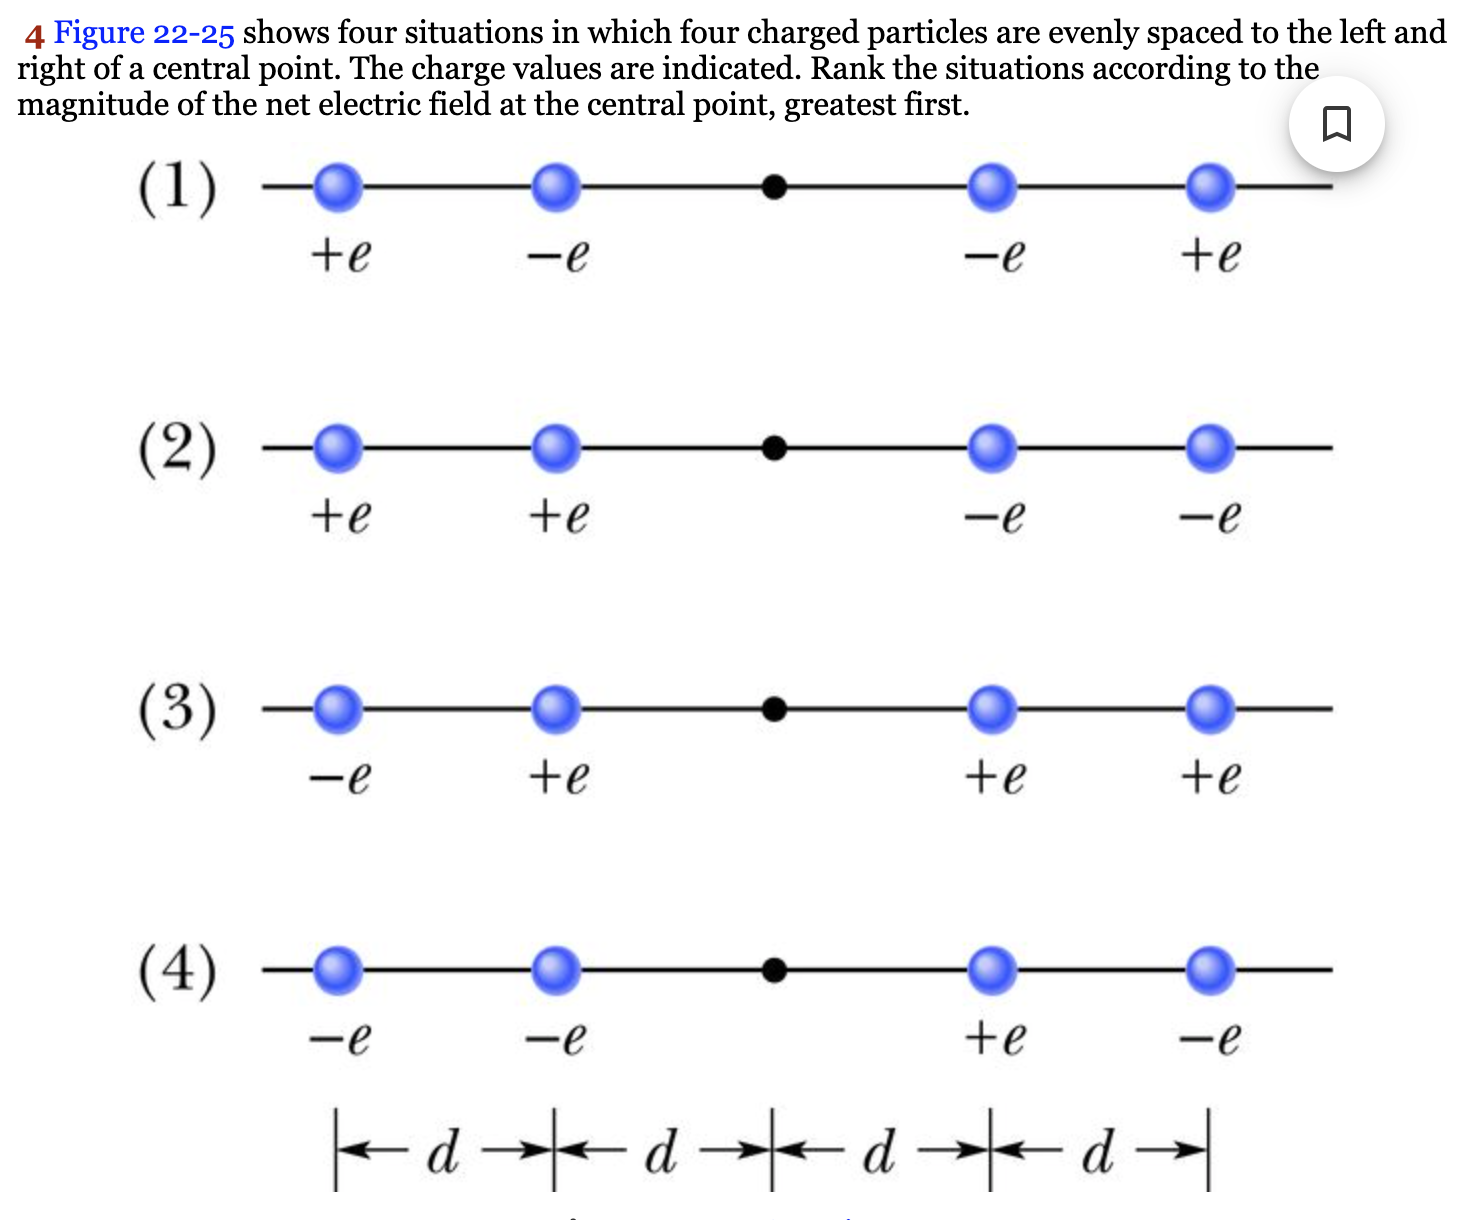
\includegraphics[width=\textwidth]{picture_3.png}

\subsection*{Solution}
We will rank them by magnitude, which is always positive. I will rank the charges in terms of "agreeing" with the direction of the majority of electric fields and "disagreeing" with the majority of electric fields.\\
Number 1 has the same charges the same distances on each side, so the magnitude is zero. This means that it will be the least.\\
Number 2 has opposite charges on each side, so the magnitude is very big. $(2) > (1)$\\
Number 3 has three agreeing charges and one disagreeing charges. This means that its net electric field is greater than zero, but not as big as (2) where they all agree. $(2) > (3) > (1)$\\
Number 4 has one disagreeing charge like number 3, but it is farther than number 3's field. This means that its field on the point has a lesser impact on it because distance is inversely proportional to field strength. As such, the magnitude is more than the magnitude of (3). \boxed{(2) > (4) > (3) > (1)}


\pagebreak
\section*{Chapter 22, Question 5}
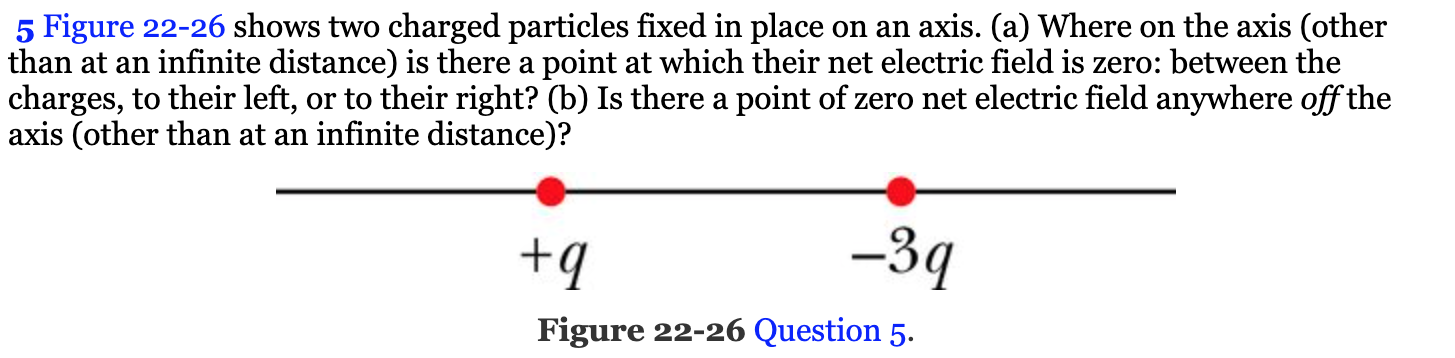
\includegraphics[width=\textwidth]{picture_4.png}

\subsection*{Solution Part (a)}
If the point charge is to the right, the closer charge being a greater charge will make the electric field always non-zero. In between the two charges, the $+q$ will push the electric field in the same direction as the $-3q$ charge will. To the left, the $-3q$ pushes it with an increasingly lower magnitude at a faster rate to which the $+q$ pushes it, so if there is a 0 point, it is \boxed{\text{to the left}}.
\begin{gather*}
    E_1 = -E_2\\
    \frac{3kq}{r^2} = \frac{kq}{(r - 1)^2}\\
    3r^2 - 6r + 3 = r^2\\
    2r^2 - 6r + 3 = 0\\
    r = \frac{3 \pm \sqrt{3}}{2}
\end{gather*}
This means that it would be $\frac{3 \pm \sqrt{3}}{2}$ times the distance between the particles to the left of the $-3q$ particle.
\pagebreak
\subsection*{Solution Part (b)}
Anywhere the electric fields cancel each other out where the above equation works when using the vector notation. We could try to calculate whether this is possible.\\
We start with the y-vectors.
\begin{gather*}
    \frac{kq}{r_1^3} + \frac{k*(-3q)}{r_2^3} = 0\\
    \frac{1}{r_1^3} = \frac{3}{r_2^3}\\
    3r_1^3 = r_2^3\\
    r_2 = r_1 \sqrt[3]{3}
\end{gather*}

We can then do what we can with the x-vectors, assuming that the charges are $s$ apart.
\begin{gather*}
    E_1 = -E_2\\
    \frac{3kq(x - s)}{r_2^3} = \frac{kqx}{r_1^3}\\
    3(x - s)r_1^3 = x r_2^3\\
    3(x - s)r_1^3 = x (r_1 \sqrt[3]{3})^3\\
    3x r_1^3 - 3s r_1^3 = 3x r_1^3\\
    x - s = x\\
    s = 0
\end{gather*}

Since the solution we got was $s = 0$, which would have to superimpose partcles and which is on the axis, there is \boxed{\text{no point}}.

\pagebreak
\section*{Chapter 22, Problem 8}
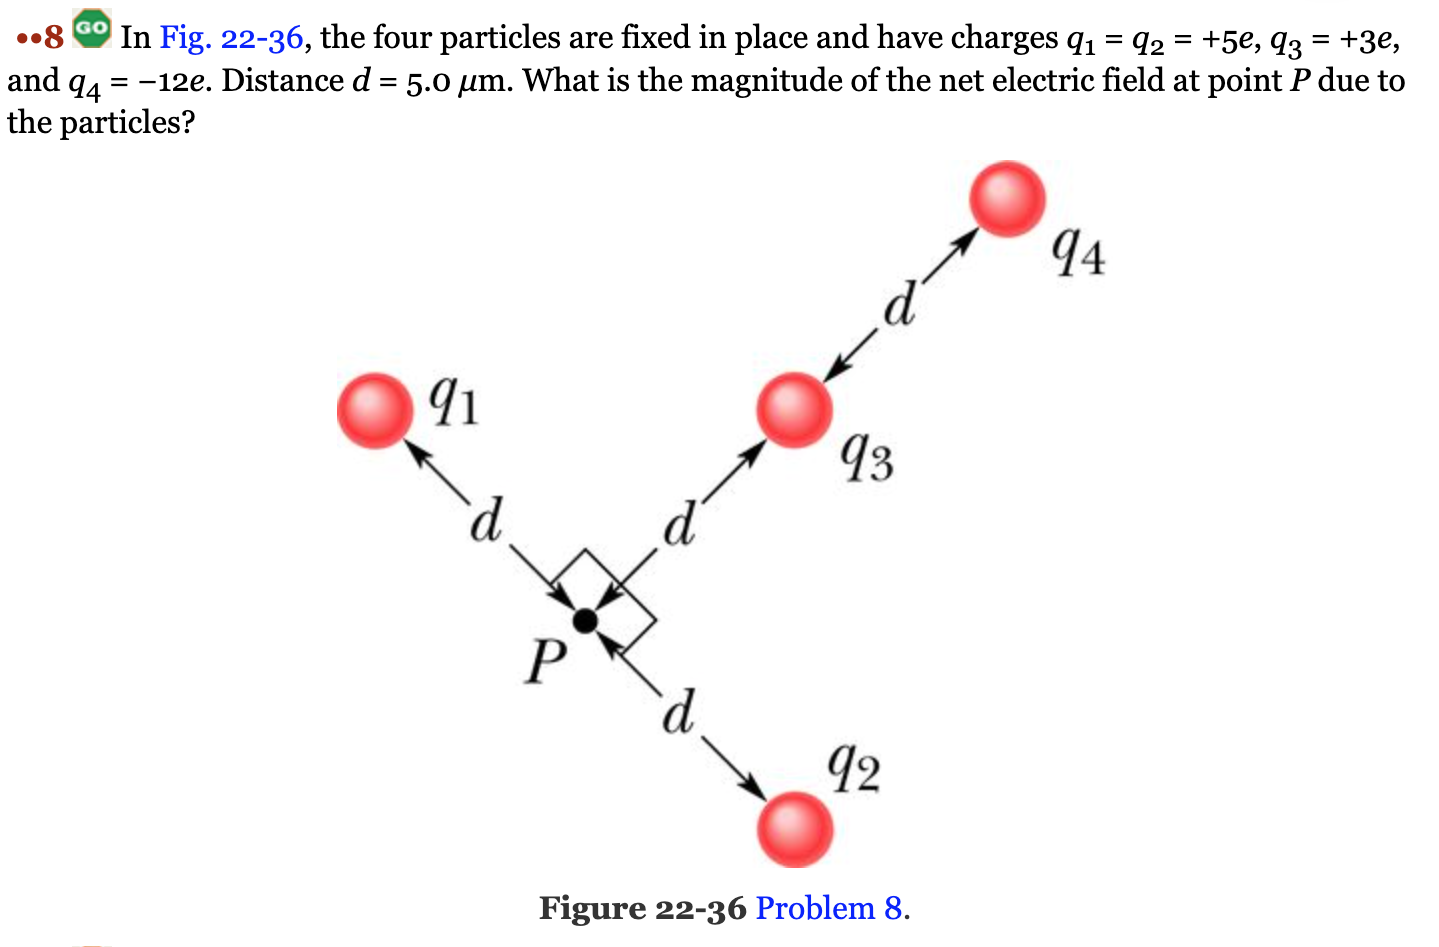
\includegraphics[width=\textwidth]{picture_5.png}

\subsection*{Solution}
First thing's first, since they're of equal charge and equaal but opposite distance on the same axis going through the point, the particles $q_1$ and $q_2$ cancel each other out, so we only need to consider particles $q_3$ and $q_4$.
\begin{align*}
    \vec{E}_P   &=  k\left(\frac{3e}{(5\times 10^{-6})^2} - \frac{12e}{(2*5\times 10^{-6})^2}\right)\\
        &=  k\left(\frac{3e}{(5\times 10^{-6})^2} - \frac{3e}{(5\times 10^{-6})^2}\right)\\
        &=  \frac{k*3e}{(5\times 10^{-6})^2}\left(1 - 1\right)\\
        &=  \boxed{0\unit{\newton/\coulomb}}
\end{align*}
I suppose that the other two particles cancel each other out as well. I will be honest, that was pretty anticlimactic. 

\pagebreak
\section*{Chapter 22, Problem 12}
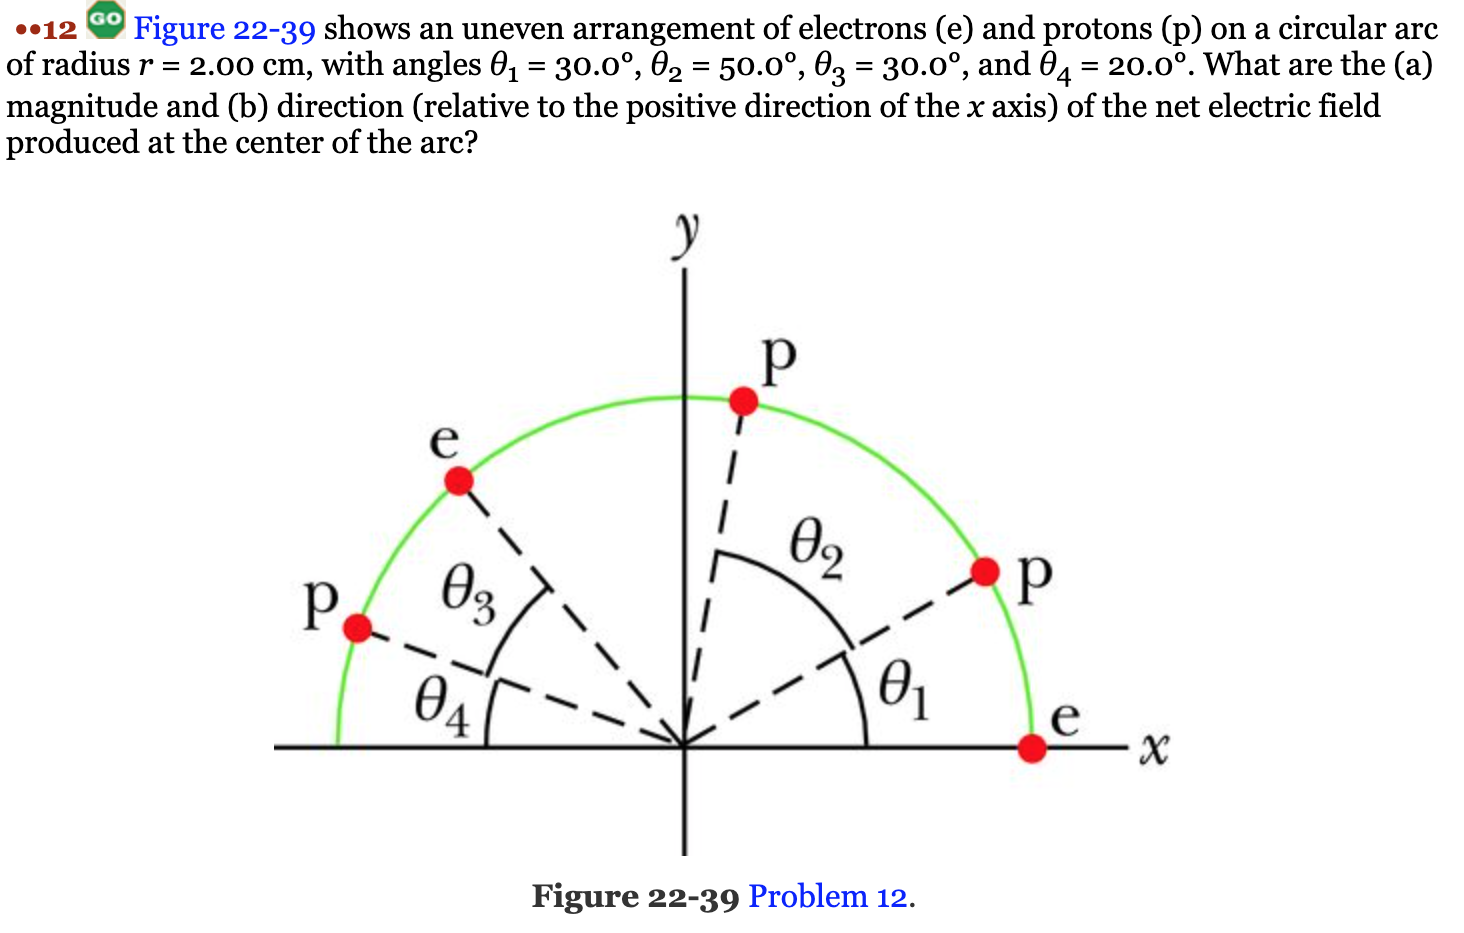
\includegraphics[width=\textwidth]{picture_6.png}

\subsection*{Solution}
We have the superposition principle and six charges, which I will number in reverst clockwise order. I will be using vector notation. We will keep the charge of a proton as $e = 1.60217663 \times 10^{-19} \unit{\coulomb}$ and the charge of an electron as $-e = -1.60217663 \times 10^{-19} \unit{\coulomb}$.
\begin{align*}
    \vec{E}_{net}   =&  \vec{E}_1 + \vec{E}_2 + \vec{E}_3 + \vec{E}_4 + \vec{E}_5 + \vec{E}_6
        =   \frac{k}{r^2}\sum_{i=1}^{6} - q_i \hat{r_i}\\
        =&  \frac{k}{0.02^2}\left(-\frac{-e}{1}\begin{pmatrix}\cos(0\unit{\degree})\\ \sin(0\unit{\degree})\end{pmatrix}
            - \frac{e}{1}\begin{pmatrix}\cos(30\unit{\degree})\\ \sin(30\unit{\degree})\end{pmatrix}
            - \frac{e}{1}\begin{pmatrix}\cos(80\unit{\degree})\\ \sin(80\unit{\degree})\end{pmatrix}\right. \\
            & \left. - \frac{-e}{1}\begin{pmatrix}\cos(130\unit{\degree})\\ \sin(130\unit{\degree})\end{pmatrix}
            - \frac{e}{1}\begin{pmatrix}\cos(160\unit{\degree})\\ \sin(160\unit{\degree})\end{pmatrix}\right)
\end{align*}

\begin{align*}
    \vec{E}_{net}   =&  \frac{ke}{0.02^2}\left(\begin{pmatrix}\cos(0\unit{\degree})\\ \sin(0\unit{\degree})\end{pmatrix}
        - \begin{pmatrix}\cos(30\unit{\degree})\\ \sin(30\unit{\degree})\end{pmatrix}
        - \begin{pmatrix}\cos(80\unit{\degree})\\ \sin(80\unit{\degree})\end{pmatrix}
        + \begin{pmatrix}\cos(130\unit{\degree})\\ \sin(130\unit{\degree})\end{pmatrix}
        - \begin{pmatrix}\cos(160\unit{\degree})\\ \sin(160\unit{\degree})\end{pmatrix}\right)\\
        =&  \frac{ke}{0.02^2} \begin{pmatrix}
            1   - \frac{\sqrt{3}}{1}    - 0.1736482 - 0.6427876    + 0.9396926\\
            0   - \frac{1}{1}           - 0.9848078 + 0.7660444    - 0.3420201
        \end{pmatrix}
        =   \frac{ke}{2^2} \begin{pmatrix}
            0.2572314\\
            -1.0607835
        \end{pmatrix}\\
        =&  \frac{(8.99 \times 10^{9})(1.60217663 \times 10^{-19})}{4 \times 10^{-4}}\begin{pmatrix} 0.2572314 \\ -1.0607835\end{pmatrix}\\
        =&  \begin{pmatrix} 9.2626259 \times 10^{-7} \\ -3.8197666 \times 10^{-6} \end{pmatrix} \unit{\newton/\coulomb}
\end{align*}

\subsubsection*{(a) Magnitude}
For the magnitude, we use the Pythagorean theorem.
\begin{align*}
    \sqrt{(9.2626259 \times 10^{-7})^2 + (-3.8197666 \times 10^{-6})^2} = \boxed{3.9304681 \times 10^{-6} \unit{\newton/\coulomb}}
\end{align*}

\subsubsection*{(b) Direction}
For the direction, we use an arccosine, keeping in mind that the vector would be in the fourth quadrant. 
\begin{equation*}
    \theta = \arccos\left(\frac{9.2626259 \times 10^{-7}}{3.9304681 \times 10^{-6}}\right)
        =   \boxed{283.6307 \unit{\degree}}
\end{equation*}


\pagebreak
\section*{Chapter 22, Problem 46}
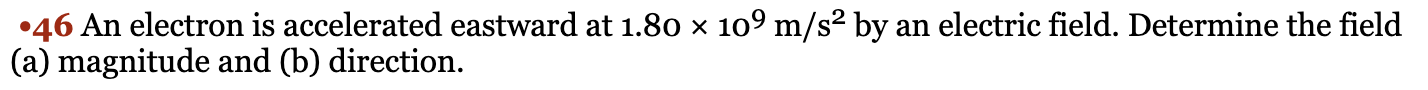
\includegraphics[width=\textwidth]{picture_7.png}

\subsection*{Solution}
The formula we have from Newton's second law is $\vec{F}_{net} = m\vec{a}$. We already have the acceleration, that being $1.80 \times 10^9 \unit{\meter/\second^2}$ eastward. We can also apply the mass of the electron ($9.1093837 \times 10^{-31} \unit{\kilo\gram}$), also keeping in mind the charge of an electron ($-1.60217663 \times 10^{-19} \unit{\coulomb}$). We can also keep in mind that $\vec{F}_{net} = q \vec{E}_{net}$
\begin{align*}
    \vec{F}_{net}   =   m\vec{a}
        &=  q \vec{E}_{net}\\
    \vec{E}_{net}   &=  \frac{m\vec{a}}{q}
        =   \frac{(9.1093837 \times 10^{-31} \unit{\kilo\gram})*(1.80 \times 10^9 \unit{\meter/\second^2})}{-1.60217663 \times 10^{-19} \unit{\coulomb}}\\
        &=  -1.02341342103 \times 10^{-2} \unit{\newton/\coulomb}
\end{align*}

a) Since we are looking for the magnitude, we take the absolute value, which is (approximately) \boxed{1.0234 \times 10^{-2} \unit{\newton/\coulomb}}.

b) Since the original charge was going eastward and the electric field is in the opposite direction, the direction is \boxed{\text{westward}}.

\end{document}